\documentclass[11pt]{article}
\usepackage{setspace}
\setstretch{1}
\usepackage{amsmath,amssymb, amsthm}
\usepackage{graphicx}
\usepackage{bm}
\usepackage[hang, flushmargin]{footmisc}
\usepackage[colorlinks=true]{hyperref}
\usepackage[nameinlink]{cleveref}
\usepackage{footnotebackref}
\usepackage{url}
\usepackage{listings}
\usepackage[most]{tcolorbox}
\usepackage{inconsolata}
\usepackage[papersize={8.5in,11in}, margin=1in]{geometry}
\usepackage{float}
\usepackage{caption}
\usepackage{esint}
\usepackage{url}
\usepackage{enumitem}
\usepackage{subfig}
\usepackage{wasysym}
\newcommand{\ilc}{\texttt}
\newcommand{\p}{\partial}
\usepackage{etoolbox}
\usepackage{algorithm}
\usepackage{changepage}
% \usepackage{algorithmic}
\usepackage[noend]{algpseudocode}
\usepackage{tikz}


\usetikzlibrary{matrix,positioning,arrows.meta,arrows}
\patchcmd{\thebibliography}{\section*{\refname}}{}{}{}
% \PassOptionsToPackage{hyphens}{url}\usepackage{hyperref}

\providecommand{\myceil}[1]{\left \lceil #1 \right \rceil }
\providecommand{\myfloor}[1]{\left \lfloor #1 \right \rfloor }

\definecolor{dkgreen}{rgb}{0,0.6,0}
\definecolor{gray}{rgb}{0.5,0.5,0.5}
\definecolor{mauve}{rgb}{0.58,0,0.82}

\lstset{frame=tb,
  language=Python,
  aboveskip=3mm,
  belowskip=3mm,
  showstringspaces=false,
  columns=flexible,
  basicstyle={\small\ttfamily},
  numbers=none,
  numberstyle=\tiny\color{gray},
  keywordstyle=\color{blue},
  commentstyle=\color{dkgreen},
  stringstyle=\color{mauve},
  breaklines=true,
  breakatwhitespace=true,
  tabsize=3
}

\begin{document}


\title{\textbf{CSDS 491: Assignment 2}}

\author{Shaochen (Henry) ZHONG, ilc{sxz517@case.edu}}

\date{Due and submitted on 03/08/2021 \\ Spring 2021, Dr. Lewicki}
\maketitle


% We've received some common questions for A1.  Here are some hints to help you go in the right direction.
%
% Q2.2: You need only prove there is a logical gap that would require an additional assumption.
%
% Q4: It is helpful to use the conjugate prior as shown in lecture.  The  normalization factor for the posterior then has the same form as the prior (but with different arguments).
%
% Q5: Remember that the data consists of event times, and the posterior is in terms of the Poisson rate parameter lambda given the number of observed data events in a given duration from 0 to T.  You only need a single Poisson likelihood combined with the prior to get the posterior.
%
% Exploration: The terms discrete and continuous refer to the variables in the model.  See the rubric for the grading criteria. Try to make your inference problems simple models of real-world situations, rather than just numerical examples.


\section*{Q1}

\section*{Q2}

\section*{Q3. Model Complexity, Free Parameters, and Simplifying Assumptions}

\subsection*{3.1.}

\begin{align*}
    p(x_1, x_2, \dots, x_N) &= p(x_1 \mid x_2, x_3, \dots, x_N) p(x_2, x_3, \dots, x_N) \\
    &= p(x_1 \mid x_2, x_3, \dots, x_N) p(x_2 \mid x_3, x_4, \dots, x_N) p(x_3, \dots, x_N) \\
    &= p(x_N) \cdot \prod_{i = 1}^{N-1} p(x_i \mid x_{i+1},  x_{i+2}, \dots, x_{N})
\end{align*}

\subsection*{3.2.}

This questions is essentially asking how many combination can we have for $\{ x_1, x_2, \dots, x_N \}$ given each $x_i$ has $K$ differrents states. As there will be $K^N$ combinations, there will be $K^N - 1$ parameters needed since the last state of the last node will not need another new parameter (it can be represent as the negation of all other states).

Similarily, we may continue upon the formula obtained in above question where $p(x_N) \cdot \prod_{i = 1}^{N-1} p(x_i \mid x_{i+1},  x_{i+2}, \dots, x_{N})$. Known that $x_N$ needs $(K-1)$ parameters to represent (since the last state can be represent as the negation of all other states) and a node with $i$ parents need $K^i$ parameters to represent.

\begin{align*}
    \sum_{i = 1}^{N} (K-1)(K^{N - i}) &= (K - 1)(K^{N - 1}) + (K - 1)(K^{N - 2}) + \dots + (K - 1)(K^0) \\
    &= (K-1) \cdot \frac{K^N - 1}{K - 1} = K^N - 1
\end{align*}

And $K^N - 1$ will be generalized as $O(K^N)$.

\subsection*{3.3.}

The $m$ root nodes each with $K$ stats will need $m(K - 1)$ parameters. The $N-m$ leaf nodes will each have $(K-1)$ parameters needed for itself and $K^m$ parameters needed for its $m$ of $K$-state parents. Thus, we will have:

\begin{equation*}
    m(K - 1 ) + (N-m)(K-1)K^m
\end{equation*}

parameters needed.

\subsection*{3.4.}

Since the formula of noisy-OR is given in a ``leaky'' fashion $p(x_i \mid \textrm{pa}({x_i})) = 1 - (1 - \mu_{i0}) \prod_{j \in \textrm{pa}(x_i)}(1 - \mu_{ij})^{x_j}$ where a $(1 - \mu_{i0})$ is involved. Each leaf nodes will have $(K-1)$ parameters needed for itself, and each of its parents will need $m^(k-1)$ parameters as each parent node has $k$ states (but since we only need a single parent at a time so we don't need another new parameter for the last state, so $k-1$). Last, we need one more parameter for the leak node $\mu_{i0}$ for each leaf node. All others remain unchanged and we have (note $K - 1 = 1$):

\begin{equation*}
    m(K-1) + (N-m)(K-1)(m^{K-1} + 1)= m + (N-m)(m + 1)
\end{equation*}

\section*{Q4. Models of Conditional Probability}


\subsection*{4.1.}

There must be at least a parent $x_j = 1$ as otherwise for $p(x_i = 1 \mid \textrm{pa}(x_i)) = 1 - (1 - \mu_{i0}) \cdot \prod_{j \in \textrm{pa}(x_i)} (1 - \mu_{ij})^0 = 1 - 1(1 - \mu_{i0})$ which will be very close to $0$; in fact, $p(x_i = 1 \mid \textrm{pa}(x_i))$ will be $0$ if we don't consider the leak node. So we know that there must be at least $x_j = 1$.\newline

This means if we have one $x_j = 1$ with a high $\mu_{ij} = \p(x_i = 1 \mid x_j = 1)$, we will have a very low $1 - \mu_{ij}$ and therefore bring the overall $p(x_i = 1 \mid \textrm{pa}(x_i))$ to be closer to zero. Since only one $x_i = x_j = 1$ with a high $\mu_{ij}$ will dramatically increase the overall output of  $p(x_i = 1 \mid \textrm{pa}(x_i))$, this works similar to the OR gate which will make $p(x_i = 1 \mid \textrm{pa}(x_i)) = 1$ with just one of its parent nodes being $1$. The noisy-OR is considered to be ``soft'' as it won't make the $p(x_i = 1 \mid \textrm{pa}(x_i))$ to be exactly 1 but only close to 1.

\subsection*{4.2.}

It is a leak node defined in the D\'{i}ez version of Leaky Noisy-OR function. It is aim to compensate the fact that in a complicate model, a $x_i$ can be 1 even if all of its parents are not 1 -- which can be roughly understand as a prior/bias base on prior knowlegde to the model.

Since we may assign a value to each $\mu_{i0}$, even if all parents of $x_i$ are zeros, we have:

\begin{align*}
    p(x_i \mid \textrm{pa}({x_i})) &= 1 - (1 - \mu_{i0}) \prod_{j \in \textrm{pa}(x_i)}(1 - \mu_{ij})^{x_j} \\
    &= 1 - (1 - \mu_{i0}) \prod_{j \in \textrm{pa}(x_i)}(1 - \mu_{ij})^0 \\
    &= \mu_{i0}
\end{align*}

Note it is only the D\'{i}ez version of leaky noisy-OR function as it was made on the assumption that the prior knowlegde will not have any effect on the output of modeled variables (the conditional output given the parents, namely all the $\mu_{ij}$s). Where Henrion considered the prior knowlegde will affect the output of all modeled variables as $p(x_i \mid \textrm{pa}({x_i})) = 1 - (1 - \mu_{i0}) \prod_{j \in \textrm{pa}(x_i)}(\frac{1 - \mu_{ij}}{1 - \mu_{i0}})^{x_j}$ where the $(1 - \mu_{i0})$ is part of every $u_{ij}$ outputs.

\subsection*{4.3.}

We may do the following transformation to the noisy-OR function and express it in a fashion of sum-of-weighted-inputs. For the ease of expression we will ignore the $1 - \mu_{i0}$ as it can be considered as a special parent and merge into to the $\prod_{j \in \{ \textrm{pa}(x_i) + x_0 \}}(1 - \mu_{ij})^{x_j}$. So we have the noisy-OR function being:

\begin{equation*}
    p(x_i \mid \textrm{pa}({x_i})) = 1 - \prod_{j \in \{ \textrm{pa}(x_i) + x_0 \}} (1 - \mu_{ij})^{x_j}
\end{equation*}

If we set $W_{ij} = - \ln(1 - \mu_{ij})$, we may express the nosiy-OR as (note for all $j$ we have $j \in \{ \textrm{pa}(x_i) + x_0 \}$):

\begin{align*}
    p(x_i \mid \textrm{pa}({x_i})) &= \rho (\sum_j W_{ij} \cdot x_{j}) \\
    \rho(z) &= 1 - e^{-z}
\end{align*}

We may confirm this is equivalent to the original noisy-OR function as:

\begin{align*}
    p(x_i \mid \textrm{pa}({x_i})) &= 1 - e^{-\sum_j W_{ij} \cdot x_{j}} \\
    &=1 - \frac{1}{e^{\sum_j -\ln(1 - \mu_{ij}) x_j}} \\
    &= 1 - \frac{1}{\prod_j \frac{1}{(1 - \mu_{ij}) ^ {x_j}}} \\
    &= 1 - \prod_j (1 - \mu_{ij})^{x_j}
\end{align*}

So essentially, we have the noisy-OR and sigmoid $\sigma(z) = \frac{1}{1 + e^{-z}} = 1 - \sigma(-z)$ both being a transformation function of a sum of weighted inputs. However, the sigmoid function is more general as is can take negative weights for $W_ij$, where for noisy-OR it can't since $W_{ij} = - \ln(1 - \mu_{ij})$. Moreover, noisy-OR can only take weights in the range of $(-\ln(0), -\ln(1)]$, where sigmoid can take any value to be its weights.

Due to the weight limitation issue, sigmoid can certainly compute unique functions where noisy-OR can't. But for model which needs extreme probablity (need $\{0, 1 \}$ as outputs), sigmoid function might not be applied due to it will need some extremely large negative/positive weights to bring the $\sigma(z)$ to 0 or 1. This can often be a problem if a model was operating base on the assumption of noisy-OR, and I will show one example in the below question where noisy-OR works but sigmoid doesn't; where the probablity output of the model is exactly like the prediction of noisy-OR.


\subsection*{4.4.}

First for a model which sigmoid works but noist-OR doesn't, the AND gate can be a perfect example where we have (where $x_{j1}, x_{j2}$ are parent nodes of $x_i$):

\begin{table}[H]
    \centering
    \begin{tabular}{ c  c | c }
        \hline
        $x_{j1}$ & $x_{j2}$ & $x_i$ \\
        \hline
        0 & 0 & 0 \\
        0 & 1 & 0 \\
        1 & 0 & 0 \\
        1 & 1 & 1
    \end{tabular}
\end{table}

To model this distribution with noisy-OR function, we have (note we ignore the leak node here to simplify the expression):

\begin{align*}
    p(x_i = 1 \mid x_{j1} = 0, x_{j2} = 0) &= 1 - (1 - p(x_i = 1 \mid x_{j1} = 0))^{0} \cdot (1 - p(x_i = 1 \mid x_{j2} = 0))^{0} = 0 \\
    p(x_i = 1 \mid x_{j1} = 0, x_{j2} = 1) &= 1 - (1 - p(x_i = 1 \mid x_{j1} = 0))^{0} \cdot (1 - p(x_i = 1 \mid x_{j2} = 1))^{1}\\ &= 1 - \frac{1}{2}= \frac{1}{2} & \text{Should be 0}\\
    p(x_i = 1 \mid x_{j1} = 1, x_{j2} = 0) &= 1 - (1 - p(x_i = 1 \mid x_{j1} = 1))^{1} \cdot (1 - p(x_i = 1 \mid x_{j2} = 0))^{0} \\ &= 1 - \frac{1}{2}= \frac{1}{2} & \text{Should be 0}\\
    p(x_i = 1 \mid x_{j1} = 1, x_{j2} = 1) &= 1 - (1 - p(x_i = 1 \mid x_{j1} = 1))^{1} \cdot (1 - p(x_i = 1 \mid x_{j2} = 1))^{1} \\ &= 1 - \frac{1}{2} \cdot \frac{1}{2}= \frac{3}{4} & \text{Should be 1}    % p(x_i = 1 \mid \textrm{pa}(x)) &= 1 - \frac{1}{2} \cdot \frac{1}{2}= \frac{3}{4} & \text{Should be $\frac{1}{4}$}
\end{align*}

As shown, the noisy-OR cannot model this system accurately, and this can't be solved by introducing a leak node -- since for the same $x_i$, the output answer has a different diffrence to the desired answer.\newline

\noindent However, if we use the sigmoid function to model this distribution, we may view the three neurons (events) as following:

\begin{figure}[H]
    \centering
    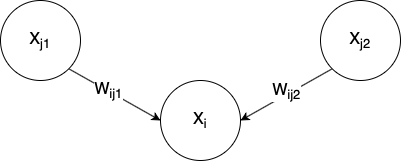
\includegraphics[width=0.6\linewidth]{{fig/p4.4}.png}
\end{figure}

And we may set $W_{ij1} = W_{ij2} = m$ and set the bias of $x_i$ to be $-1.5m$; where such $m$ must be large enough such as $\sigma(0.5m) \approx 1$. Now to calculate the probablity outputs:

\begin{align*}
    p(x_i = 1 \mid x_{j1} = 0, x_{j2} = 0) &= \sigma(0 - 1.5m) \approx 0 \\
    p(x_i = 1 \mid x_{j1} = 0, x_{j2} = 1) &= \sigma(1m - 1.5m) \approx 0 \\
    p(x_i = 1 \mid x_{j1} = 1, x_{j2} = 0) &= \sigma(1m - 1.5m) \approx 0 \\
    p(x_i = 1 \mid x_{j1} = 1, x_{j2} = 1) &=  \sigma(2m - 1.5m) \approx 1
\end{align*}

Clearly sigmoid can model this distribution as desired. This is because in sigmoid we can take an arbitrarily large weight between neurons (in this case, $m$) but we can't do such thing in noisy-OR. \newline


\noindent However, there are also distributions that can only be nicely modeled by noisy-OR but not sigmoid. Intuitively, a distribution that follows noisy-OR must be modeable by the noist-OR function; and here's an example of how a distribution follows noisy-OR assumptions can't be modeled by sigmoid.

In the above section we already established that the noisy-OR function can also be expressed as sum-of-weighted-inputs:

\begin{align*}
    p(x_i \mid \textrm{pa}({x_i})) &= \rho (\sum_j W_{ij} \cdot x_{j}) \\
    \rho(z) &= 1 - e^{-z}
\end{align*}

So if we reuse the above diagram, but set $W_{ij1} = -\ln(1 - \mu{ij1})$ and $W_{ij2} = -\ln(1 - \mu{ij2})$, we may have a distribution of:

\begin{table}[H]
    \centering
    \begin{tabular}{ c  c | c }
        \hline
        $x_{j1}$ & $x_{j2}$ & $p(x_i)$ \\
        \hline
        0 & 0 & 0 \\
        0 & 1 & $1-e^{-1}$ \\
        1 & 0 & $1-e^{-1}$ \\
        1 & 1 & $1-e^{-2}$
    \end{tabular}
\end{table}

It is trivial to show that this distribution can be modeled by the noisy-OR function as it is defined with respect to noisy-OR. So the only thing left is to show that this distribution cannot be nicely modeled by the sigmoid function.

However, this is an impossible task because:

\begin{itemize}
    \item To have $p(x_i  \mid x_{j1} = 0, x_{j2} = 0) = 0$ we must have very large and negative sum-of-weighted-inputs $z$ to bring $\sigma(z - \text{}) \approx 0$. This can be done by setting a very large and negative bias on $x_i$, like $-m$.
    \item To have $p(x_i \mid x_{j1} = 0, x_{j2} = 1), p(x_i  \mid x_{j1} = 1, x_{j2} = 0) = 1-e^{-1}$, since $1-e^{-1}$ is a positive value, we must have the $W_{ij1}, W_{ij2}$ to be greater than the absolute value of the bias $|-m|$ so that we will have $\sigma(W_{ij1} - m)$ or $\sigma(W_{ij2} - m)$ to be $\geq 0$. This means $W_{ij1}, W_{ij2}$ must be some significantly large positive value that is $> m$.
    \item Since we have established that $W_{ij1}, W_{ij2}$ must be some significantly large positive value that is $> m$. For $p(x_i \mid x_{j1} = 1, x_{j2} = 1)$ with the sigmoid function we must have $\sigma(z = W_{ij1} + W_{ij2} - m)$; where such $z$ is guaranteed to be $>m$ and we know that $\sigma(m) \approx 1$. This will create an unavoidable confict with the purposed distribution as the output should be $1-e^{-2}$ which is $\ll 1$.
\end{itemize}

So we have showed an example distribution where the noisy-OR function works but the sigmoid function doesn't. This is because to have outputs like $\{0, 1\}$ sigmoid, we must relay on large weights and large bias; but since the distribution is defined with respect to noisy-OR, it was desiged to use with smaller weights.\newline


\noindent The second example was inspired by -- or technically, taken from (although I believe there a typo in the original text regarding $e^{-1}$ where it should be $1 - e^{-1}$) -- \href{http://www.cs.toronto.edu/~bonner/courses/2016s/csc321/readings/Connectionist%20learning%20of%20belief%20networks.pdf}{R.M. Neal, Connectionist learning of belief networks, Artificial Intelligence 56 (1992) 71–113.}


\section*{Q5}

\section*{Exploration}



\end{document}

